\section{Evaluation Results}\label{result}

This section provides quantitative results of the two case study ADC designs’ fundamental characteristics and energy-saving performance. 
The statistical data is obtained from simulation in Virtuoso’s AMS Environment. 
Although some digital modules are in behavior level written by Verilog, we argue that the power consumption of this parts can be ignored 
because these digital modules are just in need of limited dynamical currents.

\subsection{Evaluation of the SS ADCs}

The fundamental characteristics of the SS ADCs are summarized in Table~\ref{tab1}. Assuming a 512×512 pixel array, the frame rate will be 162fps.
The SNDR of SS ADCs is 23.83/46.64 dB, which means the ENOB is 3.67/7.46 bits. 
The power consumption of the SS ADCs is measured and divided by columns, 
it shows that compared to 76.2uW/column for high-precison conversion, only 40.8uW/column is needed for low-precison conversion, reduced by almost a half. 
A more specific energy analysis is presented in Fig.~\ref{SSresults1}. 
As we can see, most parts of the power consumption are taken up by the column-parallel comparators and output buffer of the ramp generator, 
both of which can be power gated effectively for low-precison conversion. 
The related quantity results is presented in Fig.~\ref{SSresults2}, 
where the peripheral circuits include a bandgap and voltage divider, some level-shift circuits and global buffers.

\begin{table}[htbp]
	\caption{Performance of the SS ADCs}
	\begin{center}
		\begin{tabular}{|c|c|}
			\hline
			\textbf{Prameter}& \textbf{Value} \\
			\hhline{|==|}
			\textbf{Process}& 65nm \\
			\hline 
			\textbf{Supply voltage}& 2.5/1.2 V \\
			\hline
			\textbf{Clock Frequency}&	25MHz \\
			\hline
			\textbf{Architecture}&	SS \\
			\hline
			\textbf{Quantization bits}&	4/8 bits\\
			\hline
			\textbf{Conversion time}&	12.04us \\
			\hline
			\textbf{Number of parallel columns}&	512 \\
			\hline
			\textbf{Throughput (samples per second)}&	42.5M \\ 
			\hline
			\textbf{Power (per column)}&	40.8/76.2 uW \\
			\hline
			\textbf{SNDR}& 23.83/46.64 dB@ 8.44 kHz\\
			\hline
			\textbf{ENOB}& 3.67/7.46 bits\\
			\hline
			\textbf{FOM$^{\mathrm{a}}$}& 38.59/5.21 pJ/step\\
			\hline
			\multicolumn{2}{l}{$^{\mathrm{a}}\textbf{FOM}=(\textbf{Power}\ast \textbf{Conversion}\ \textbf{time})/2^{\textbf{ENOB}}$ }	    
		\end{tabular}
		\label{tab1}
	\end{center}
\end{table}

\begin{figure}[htbp]
	\centerline{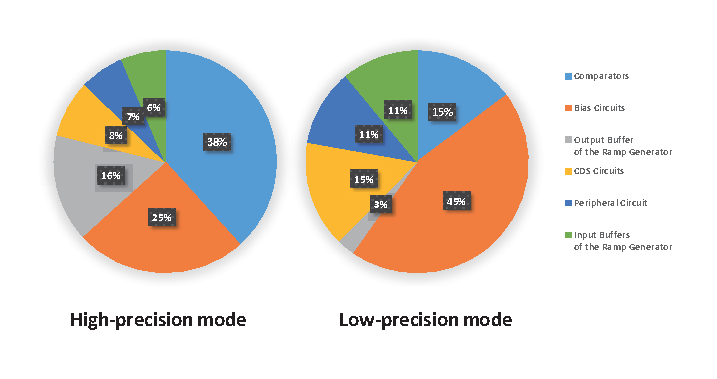
\includegraphics[width=3.5in]{./Figures/SSResults1.eps}}
	\caption{Power Distribution of the SS ADCs.}
	\label{SSresults1}
\end{figure}

\begin{figure}[htbp]
	\centerline{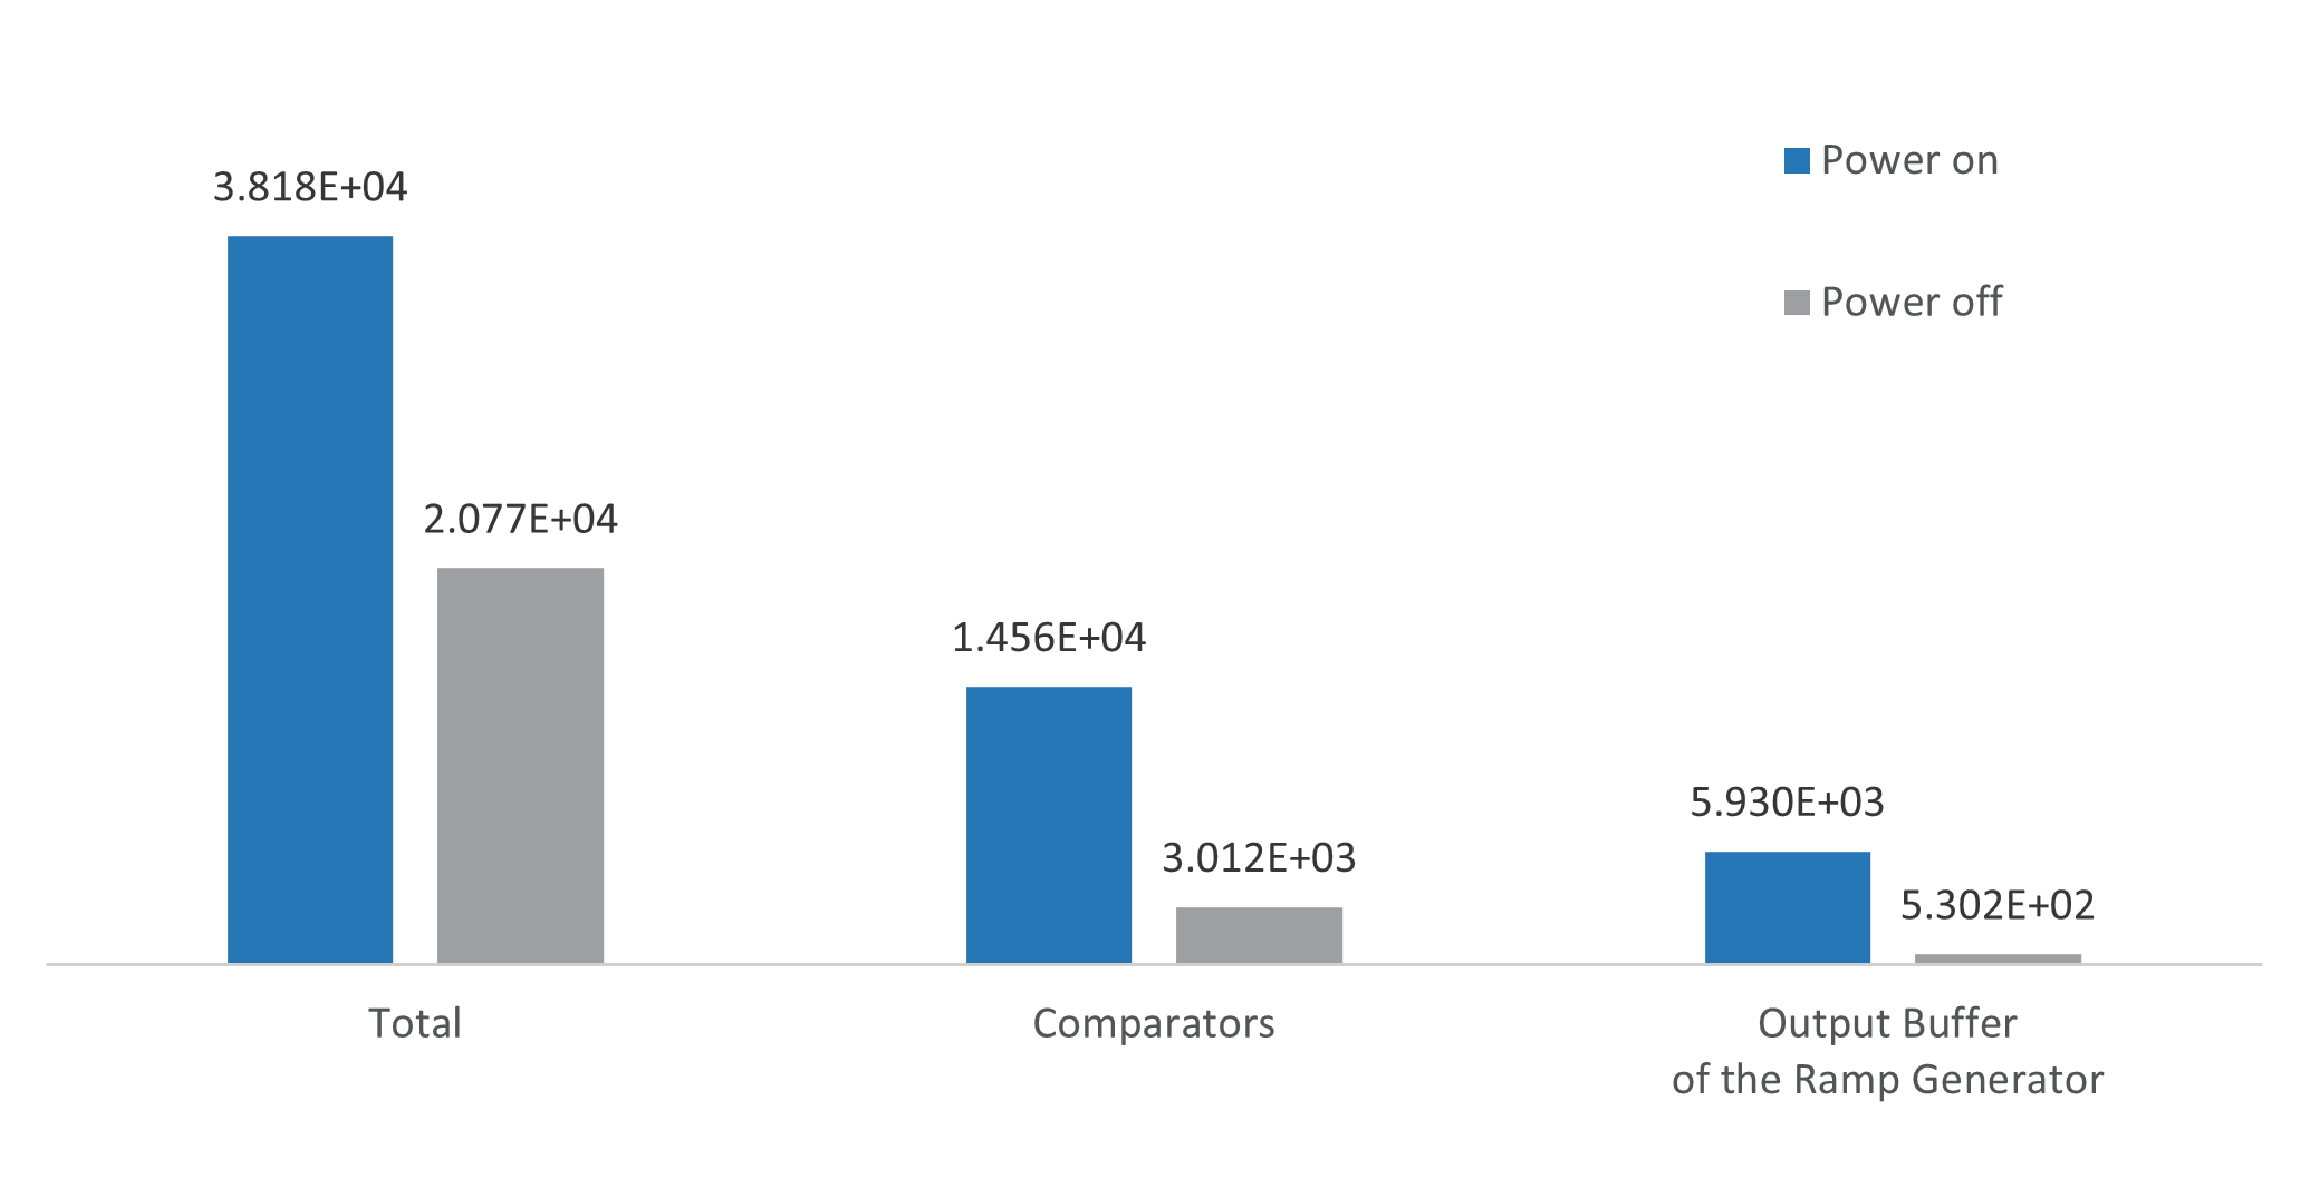
\includegraphics[width=3.5in]{./Figures/SSResults2.eps}}
	\caption{Power Saving Results of the SS ADCs.}
	\label{SSresults2}
\end{figure} 

\subsection{Evaluation of the SAR/SS ADCs}

The fundamental characteristics of the SAR/SS ADCs are summarized in Table~\ref{tab2}. 
While the throughput is set similar to the SS ADCs, fewer steps is required in the SAR/SS ADCs, where 1 conversion step counts for 2 clock periods. 
The SNDR is 24.25/57.87 dB and the ENOB is 3.74/9.32 bits, consistent with the design specifications. 
The power consumption is 256.1uW/column for high-precison conversion and 137.1uW/column for low-precison conversion, respectively. 
According to the energy analysis presented in Fig.~\ref{SARresults1}, most parts of the SAR/SS ADCs' power consumption 
are taken up by the column-parallel buffers of reference voltages in the sub-ADCs.
For low-precison conversion, the energy of the SAR/SS ADCs can also be saved to nearly half. 
The related quantity results is presented in Fig.~\ref{SARresults2}.

\begin{table}[htbp]
	\caption{Performance of the SAR/SS ADCs}
	\begin{center}
		\begin{tabular}{|c|c|}
			\hline
			\textbf{Prameter}& \textbf{Value} \\
			\hhline{|==|}
			\textbf{Process}& 65nm \\
			\hline 
			\textbf{Supply voltage}& 2.5/1.2 V \\
			\hline
			\textbf{Clock Frequency}&	20MHz \\
			\hline
			\textbf{Architecture}&	SAR/SS \\
			\hline
			\textbf{Quantization bits}&	4/10 bits \\
			\hline
			\textbf{Conversion time (us)}&	10.1us \\
			\hline
			\textbf{Number of parallel columns}&	512 \\
			\hline
			\textbf{Throughput (samples per second)}&	50.7M \\ 
			\hline
			\textbf{Power (per column)}&	137.1/256.1 uW \\
			\hline
			\textbf{SNDR}& 24.25/57.87 dB@ 10.06 kHz \\
			\hline
			\textbf{ENOB}& 3.74/9.32 bits \\
			\hline
			\textbf{FOM$^{\mathrm{a}}$}& 103.64/4.05 pJ/step\\
			\hline
			\multicolumn{2}{l}{$^{\mathrm{a}}\textbf{FOM}=(\textbf{Power}\ast \textbf{Conversion}\ \textbf{time})/2^{\textbf{ENOB}}$ }	    
		\end{tabular}
		\label{tab2}
	\end{center}
\end{table}

\begin{figure}[htbp]
	\centerline{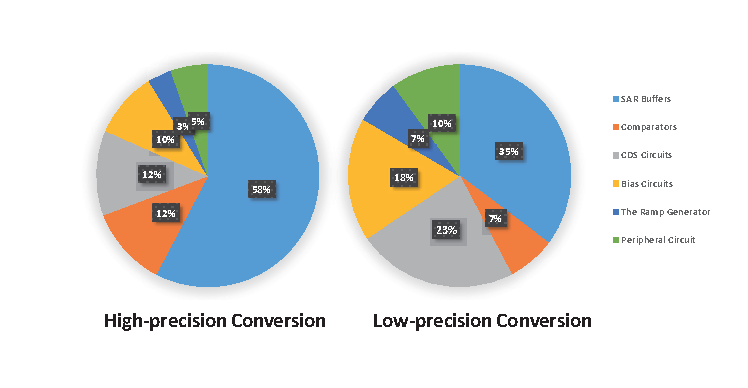
\includegraphics[width=3.5in]{./Figures/SARResults1.eps}}
	\caption{Power Distribution of the SAR/SS ADCs.}
	\label{SARresults1}
\end{figure} 

\begin{figure}[htbp]
	\centerline{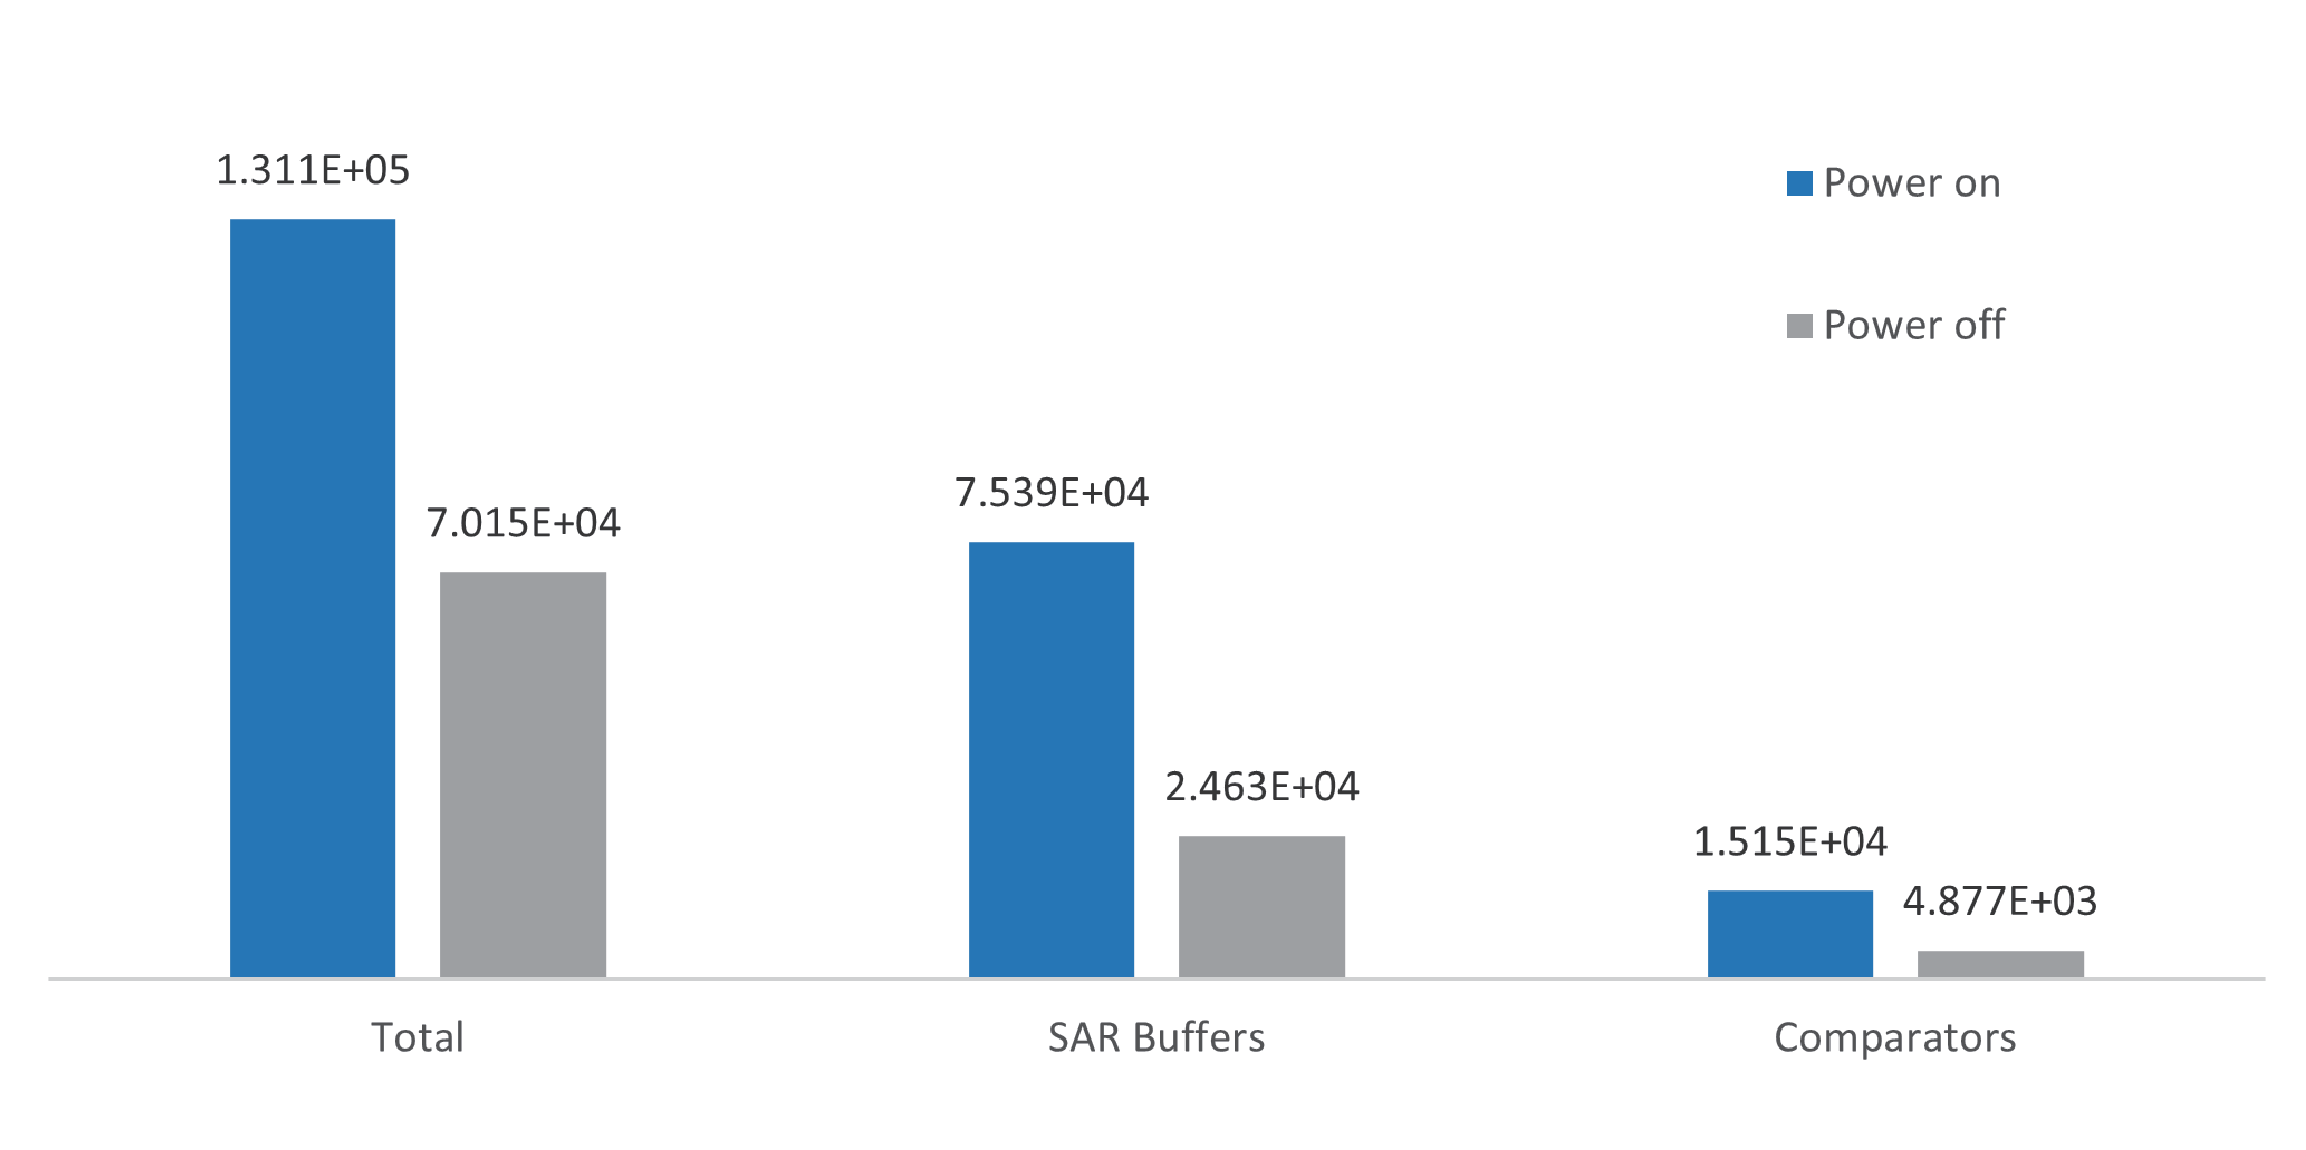
\includegraphics[width=3.5in]{./Figures/SARResults2.eps}}
	\caption{Power Saving Results of the SAR/SS ADCs.}
	\label{SARresults2}
\end{figure} 